%% Beispiel-Präsentation
\documentclass{sdqbeamer}
 
%% Titelbild
\titleimage{banner_2020_kit}

%% Gruppenlogo
\grouplogo{kitlogo_de_rgb} 

%% Gruppenname
\groupname{Team 02}

% Beginn der Präsentation

\title[Abschlusspräsentation]{Abschlusspräsentation}
\subtitle{Praktikum: Modellgetriebene Software-Entwicklung} 
\author{Dirk Neumann, Patrick Mehl, Jakob Höfker}

\date[8.\,12.\,2020]{8. Dezember 2020}

% Literatur 
 
\usepackage[citestyle=authoryear,bibstyle=numeric,hyperref,backend=biber]{biblatex}
\addbibresource{presentation.bib}
\bibhang1em

\begin{document}

%Titelseite
\KITtitleframe

%Inhaltsverzeichnis
\begin{frame}{Inhaltsverzeichnis}
\tableofcontents
\end{frame}

\section[M1: Metamodell]{M1: Meta-Modellierung}
\begin{frame}{Meta-Modellierung}
	\centering
	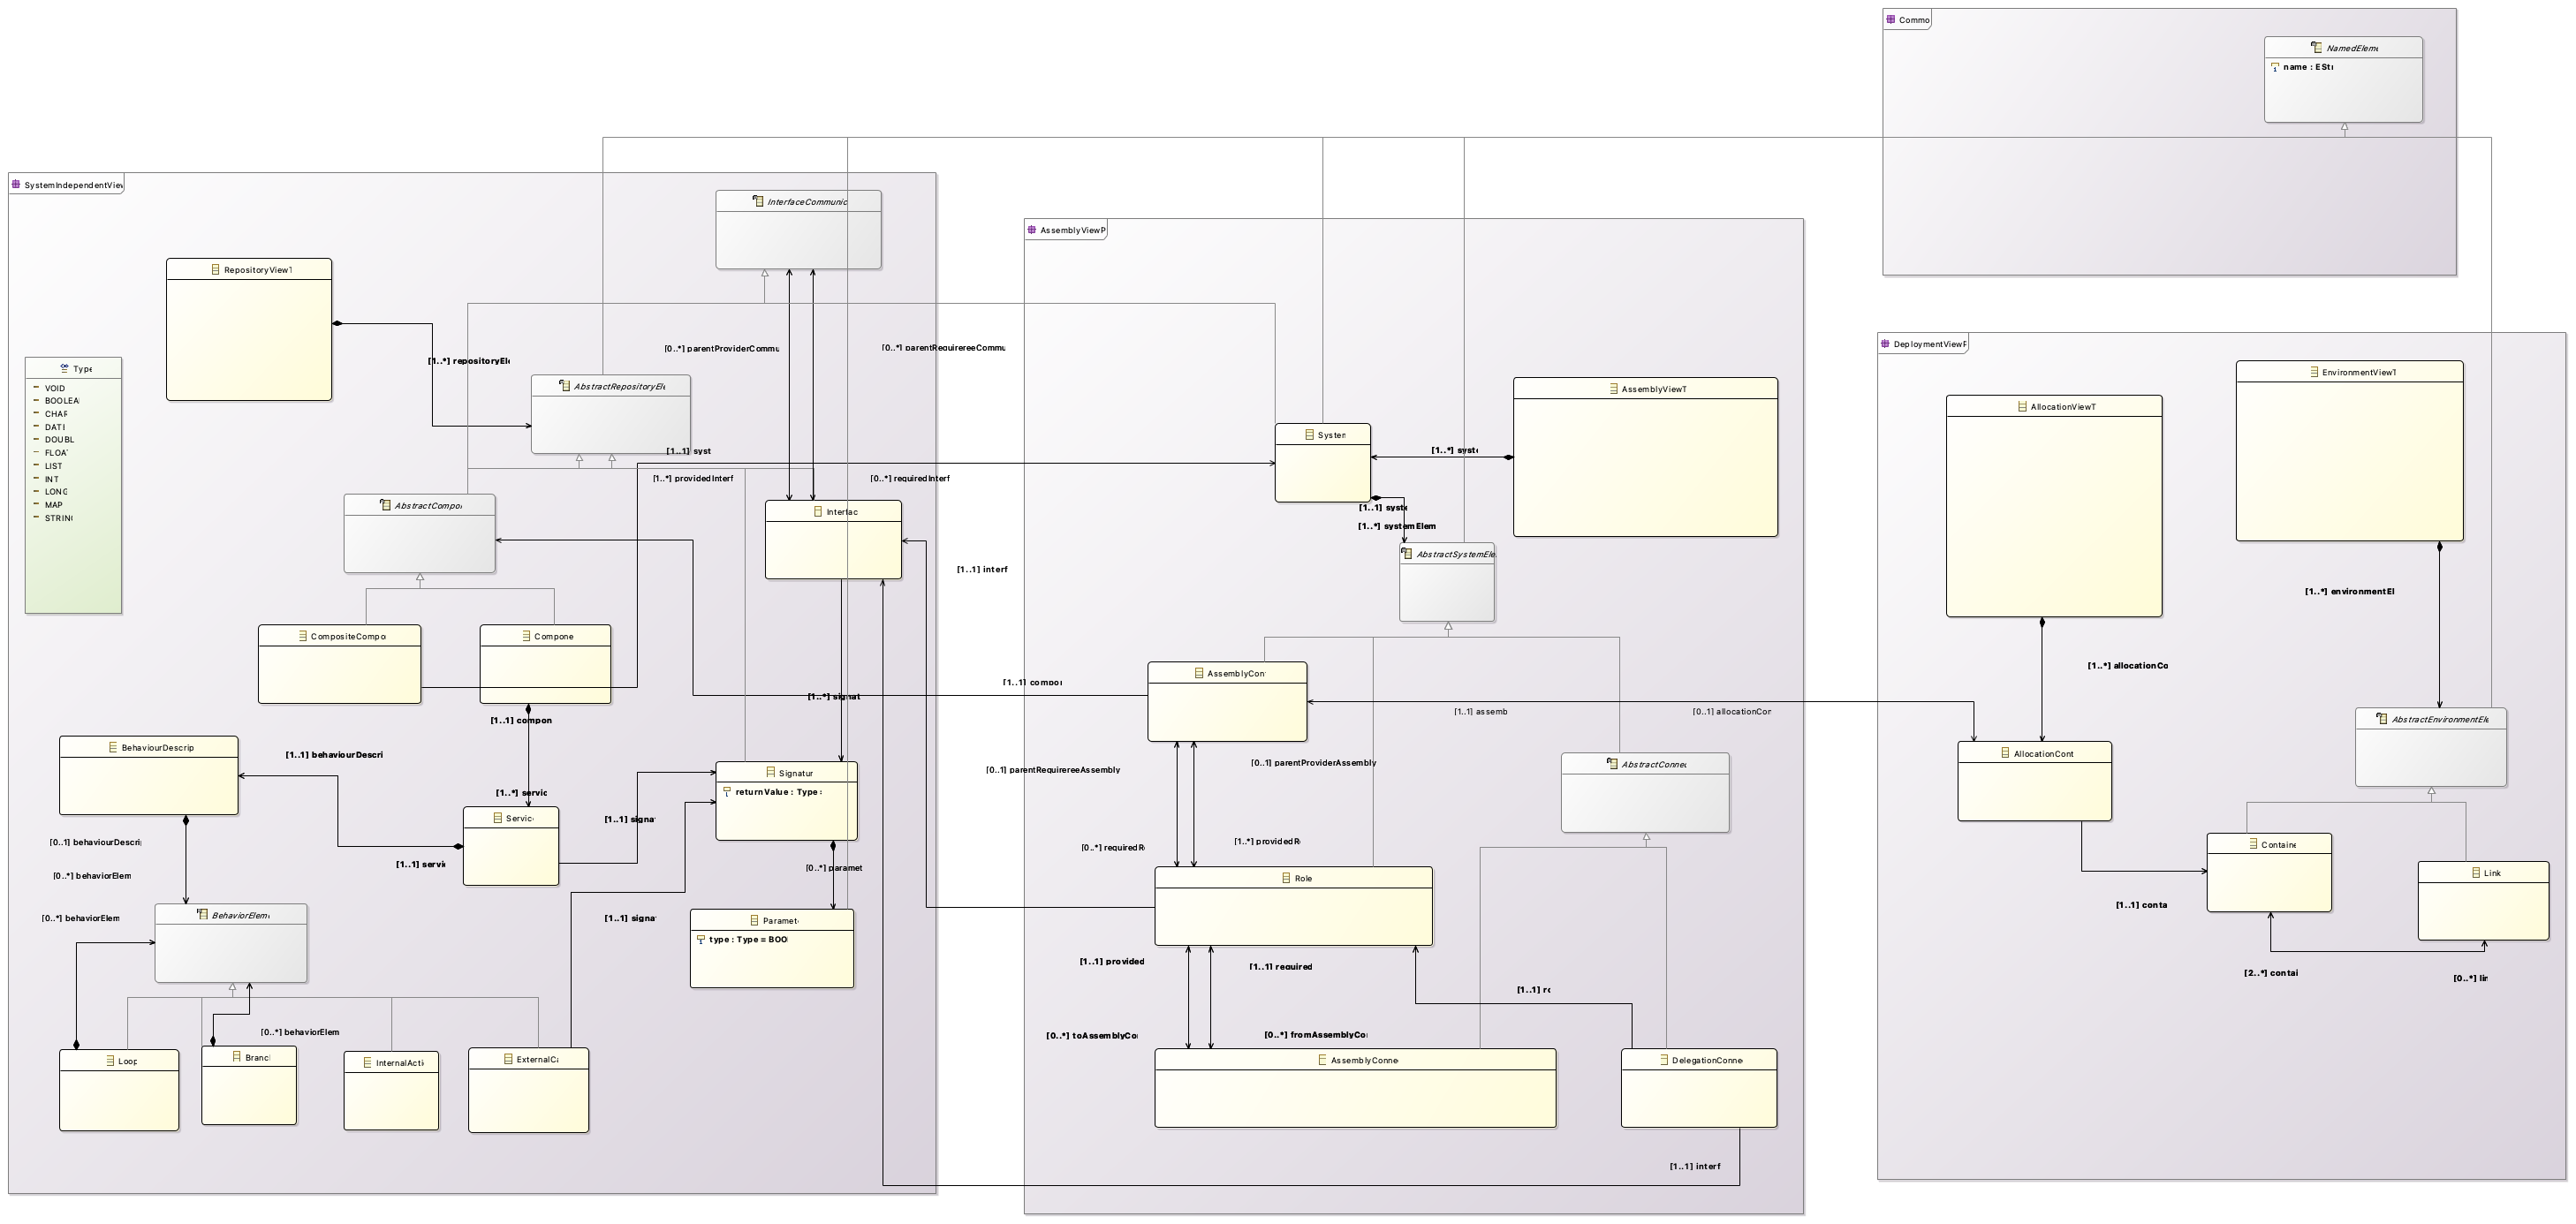
\includegraphics[height=60mm]{figures/meta-modell.png}
\end{frame}

\begin{frame}{Entwurfsentscheidungen für die Meta-Modellierung}
	\begin{itemize}
		\item Verwendung von 4 Packages
		\begin{itemize}
			\item klare Trennung der View Points
			\item Nachteil für spätere Entwicklung
		\end{itemize}
		
		\item Common Package für wiederverwendbare Elemente
		\item ENUM zur Modellierung des \texttt{Type}
		\item Verwendung von OCL
	\end{itemize}
\end{frame}
\section[M2: Xtext]{M2: Xtext - textuelle Syntax}
\begin{frame}{Xtext - textuelle Syntax}
    \begin{itemize}
        \item Ergebnis: mediastore.envvt
    \end{itemize}
	\vspace{1mm}
    \centering
	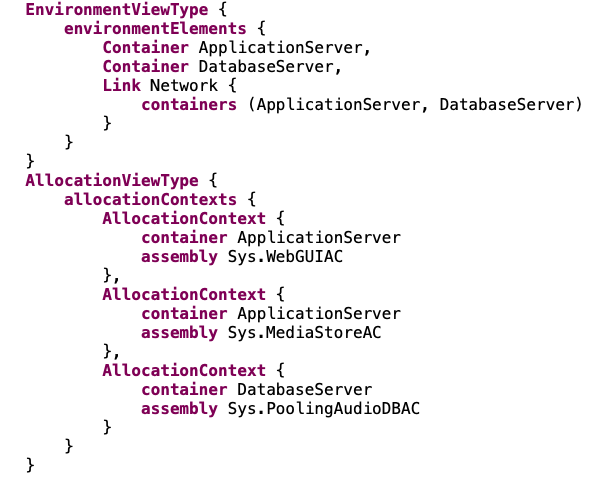
\includegraphics[height=40mm]{figures/xtext.png}
\end{frame}

\begin{frame}{Entwurfsentscheidungen und Probleme}
	\begin{itemize}
		\item import von Packages
		\begin{itemize}
            \item Lösung:
        \end{itemize}
        \item OCL Constraints
	\end{itemize}
\end{frame}
\section[M3: QVTo]{M3: QVTo - Modelltransformation}
\begin{frame}{QVTo - Modelltransformation}
	\centering
	
\includegraphics[height=10mm]{figures/modelltransformation.png}
	\begin{enumerate}
		\item Definieren von Eingabe-Modellen, Ausgabemodellen und Transformation zwischen diesen
		\item Probleme
		\begin{itemize}
			\item Verschiedene Modellierungen (Enum vs. Relation vs. Objekt)
			\item Vererbungshierarchien
			\item Weniger-explizite Informationen in SimplePalladio
		\end{itemize}
	\end{enumerate}
\end{frame}

\begin{frame}{Verschiedene Modellierungen (Enum vs. Objekt)}
	\centering
	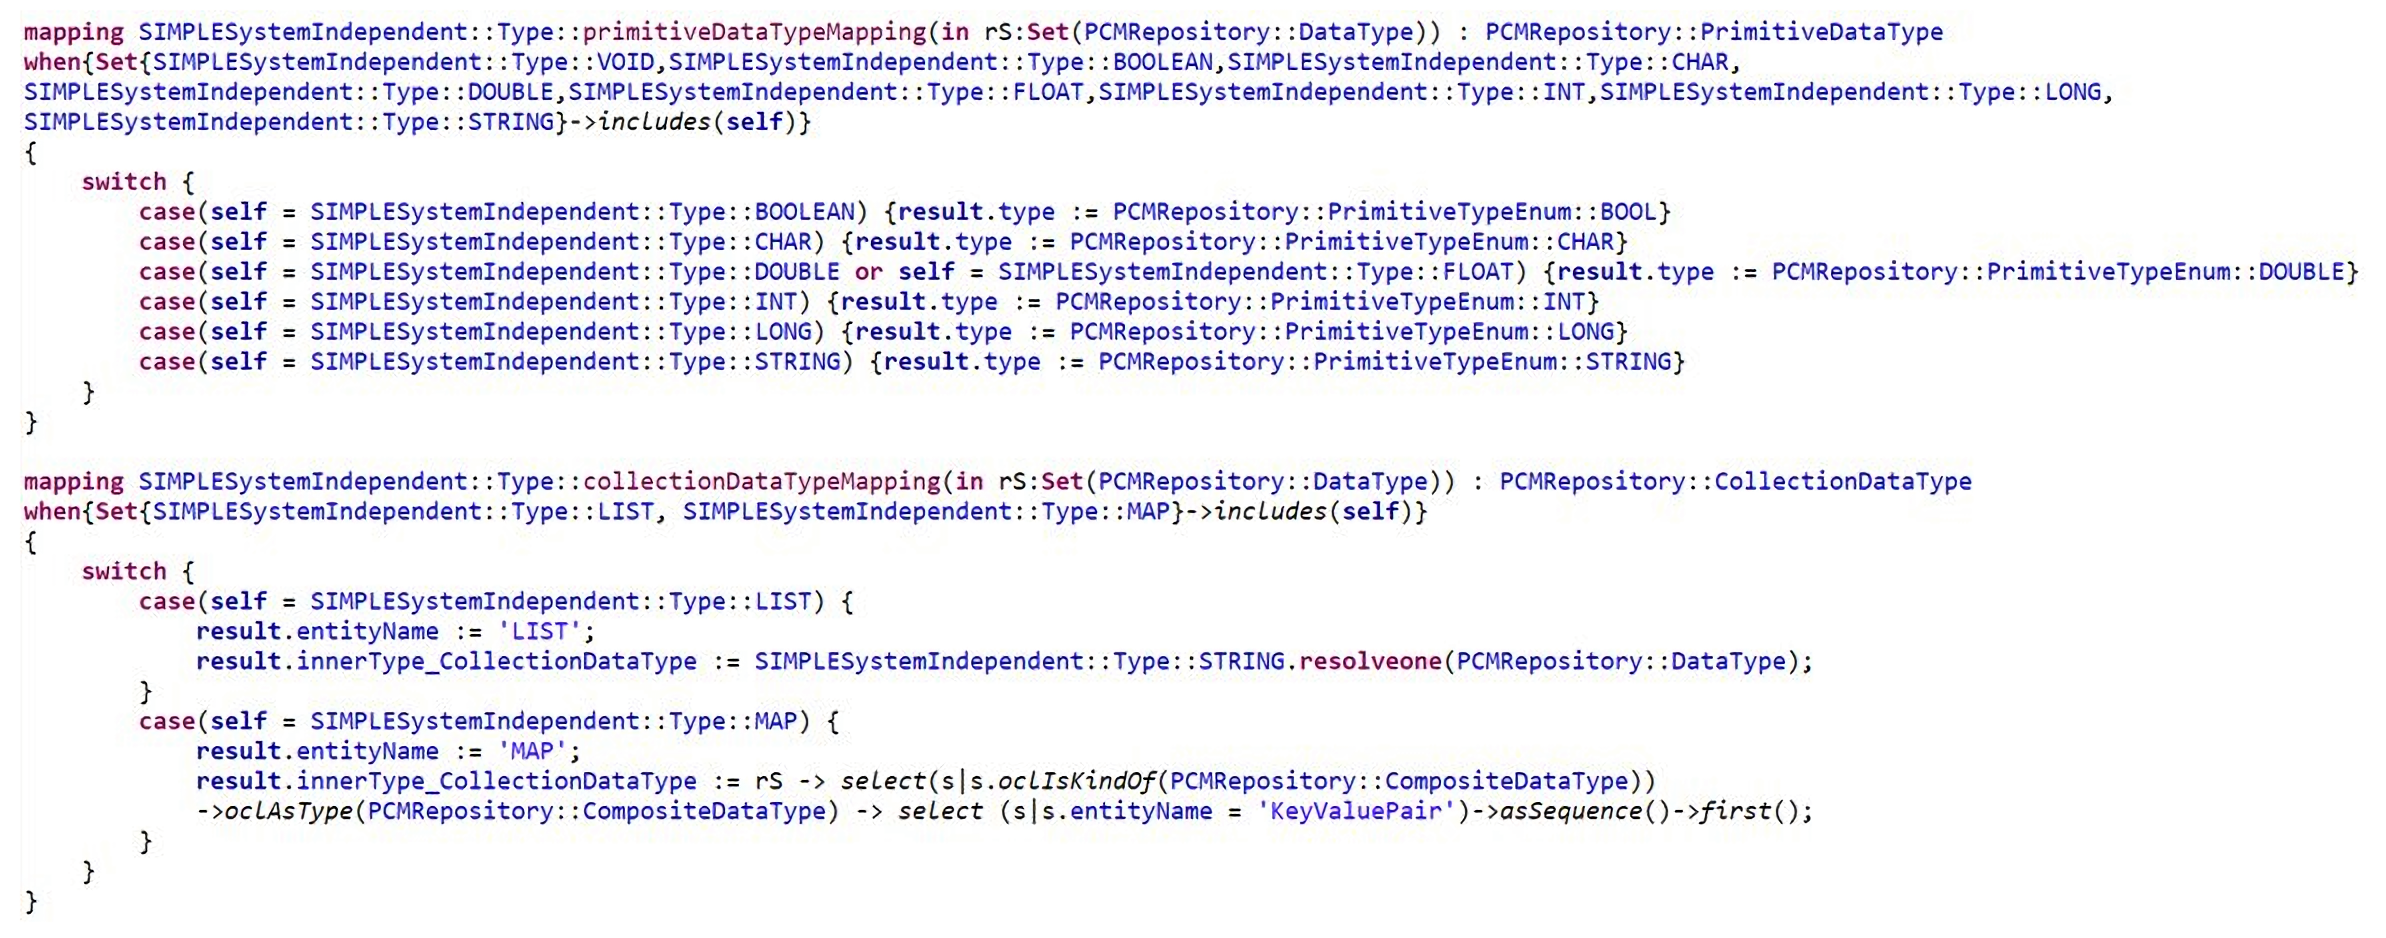
\includegraphics[height=60mm]{figures/modellierung-enum-objekt.png}
\end{frame}

\begin{frame}{Vererbungshierarchien}
	\centering
	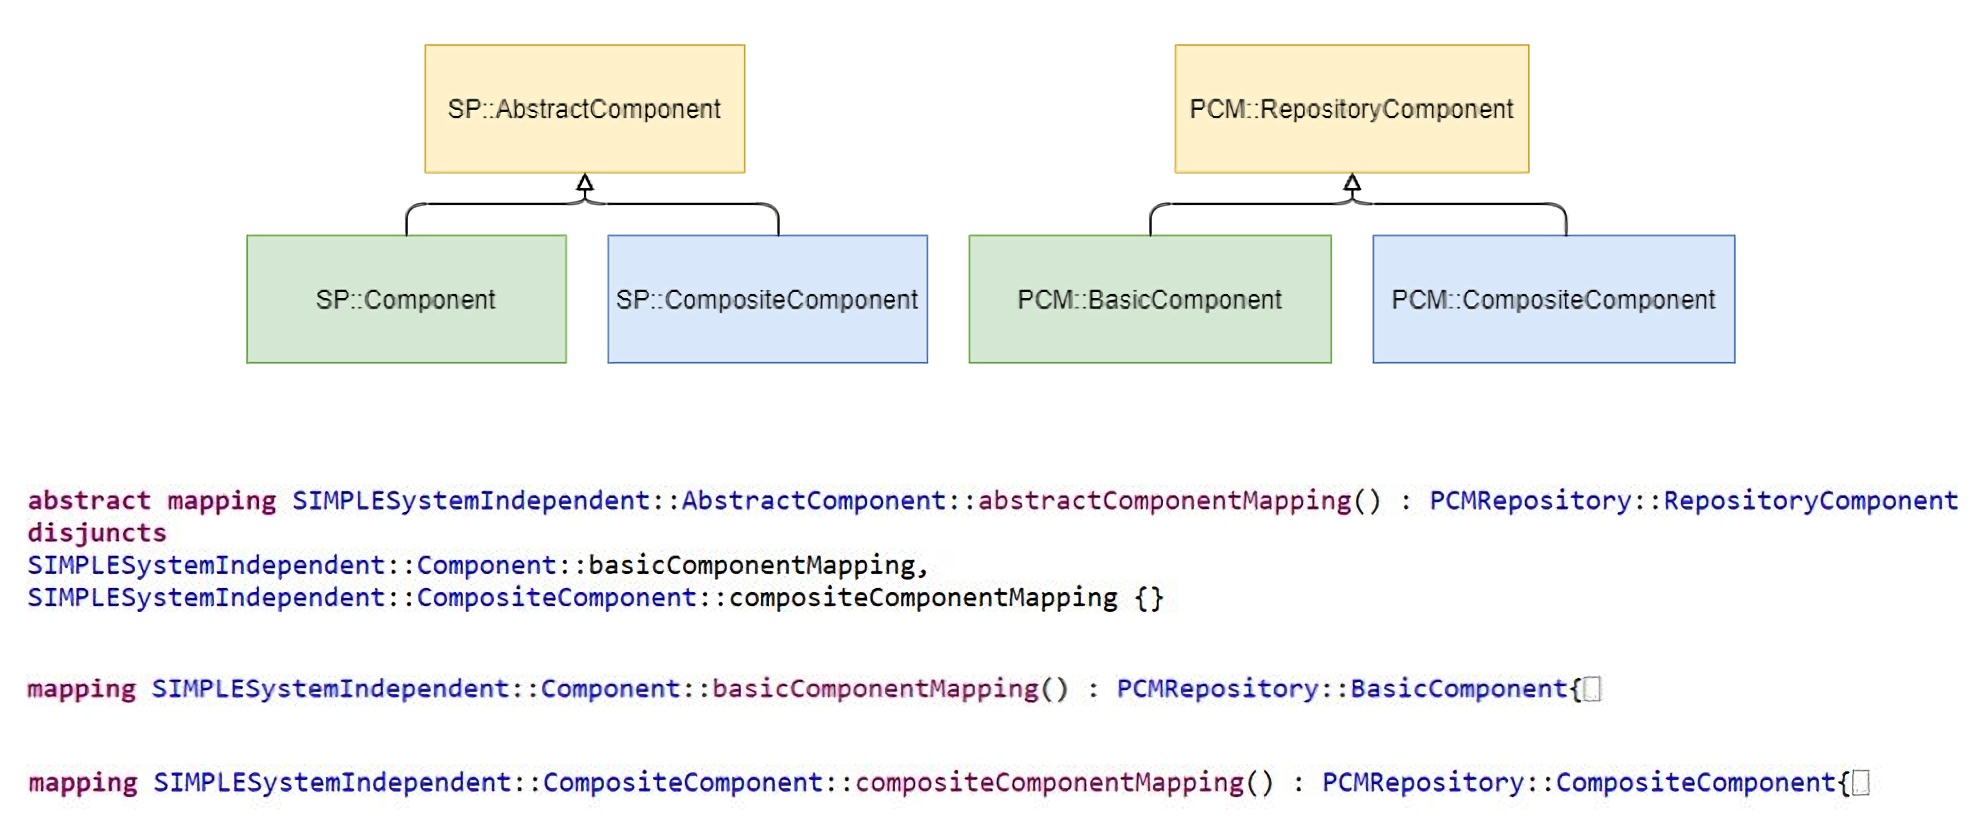
\includegraphics[height=60mm]{figures/vererbungshierachien.png}
\end{frame}

\begin{frame}{Weniger-explizite Informationen}
	\begin{enumerate}
		\item Lösung $\rightarrow$ Intermediate Objekte einführen und diese mappen
	\end{enumerate}
	\centering
	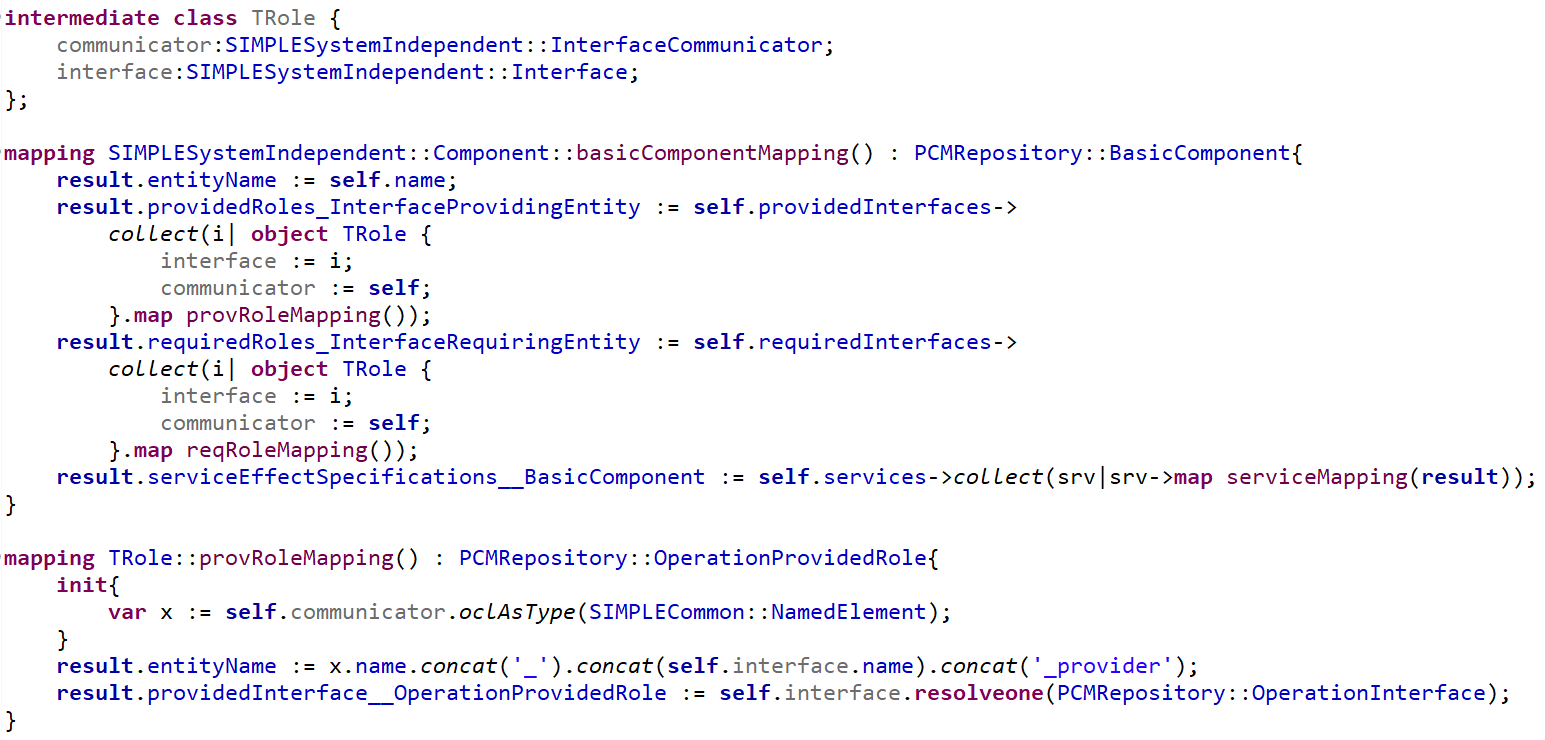
\includegraphics[height=50mm]{figures/intermediate-objekte.png}
\end{frame}
\section[M4: Xtend]{M4: Xtend - Code-Generierung}
\begin{frame}{Code-Generierung mit Xtend}
	\vspace{-5mm}
	\begin{columns}
		\column{.5\textwidth}
		\begin{contentblock}{}
			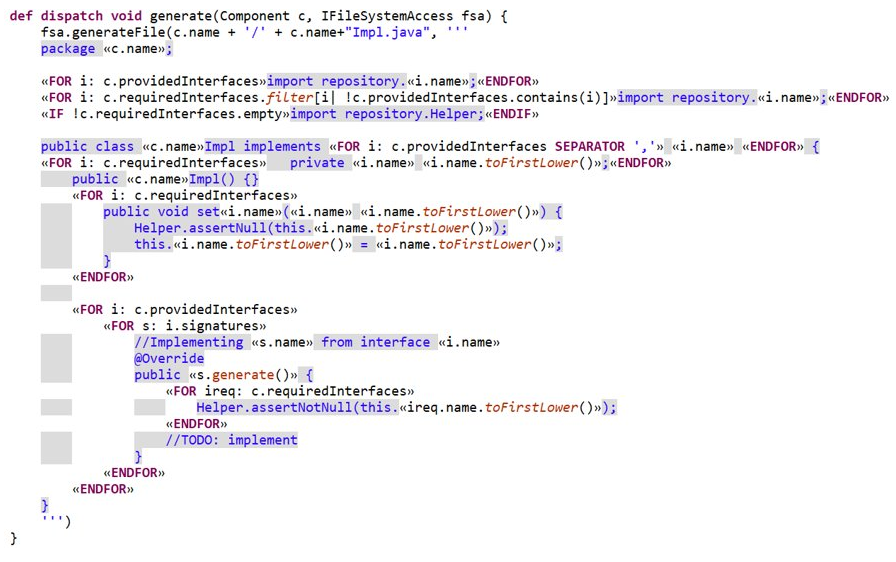
\includegraphics[height=60mm]{figures/xtend.png}
		\end{contentblock}
		\column{.5\textwidth}
		\begin{contentblock}{}
			\begin{itemize}
				\item Beispielhafte Erzeugung des Quellcodes für die DBCacheImpl-Datei mit Attributen und Methoden-Templates
				\item Generierung von \texttt{DBCache/DBCacheImpl.java}
			\end{itemize}
		\end{contentblock}
	\end{columns}
\end{frame}

\begin{frame}{Entwurfsentscheidungen bei der Code-Generierung}
	\begin{enumerate}
		\item Erzeugung der Klassen in siblings-Packages anstatt in respository-Package 
	\end{enumerate}
\end{frame}

\begin{frame}{Probleme bei der Code-Generierung}
	\begin{enumerate}
			\item OCL Constraints konnten nicht aufgelöst werden
			\begin{itemize}
				\item Deaktivierung der OCL-Validierungq
			\end{itemize} 
	\end{enumerate}
\end{frame}
\section[M5: Sirius]{M5: Sirius - grafischer Editor}
\begin{frame}{Sirius - grafischer Editor}
	\vspace{-5mm}
	\begin{columns}
		\column{.5\textwidth}
		\begin{contentblock}{}
			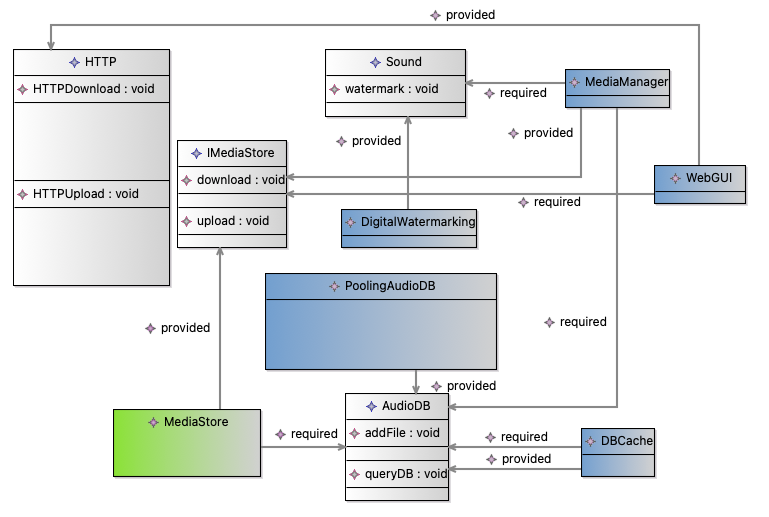
\includegraphics[width=86mm]{figures/sirius.png}
		\end{contentblock}
		\column{.5\textwidth}
		\begin{contentblock}{}
			\begin{itemize}
				\item graues Element: Interface
				\item grünes Element: Composite Component
				\item blaues Element: Component
				\item required Edge: z.B. Component required Interface 
				\item provided Edge: z.B. Component provided Interface
			\end{itemize}
		\end{contentblock}
	\end{columns}
\end{frame}

\begin{frame}{Entwurfsentscheidungen beim grafischen Editor}
	\begin{itemize}
		\item Parameter werden als Liste innerhalb von Signaturblöcken dargestellt
	\end{itemize}
\end{frame}
\section{Evaluation}
\begin{frame}{Evalutation}
	\begin{itemize}
		\item 
	\end{itemize}
\end{frame}
\section{Key Learnings}
\begin{frame}{Key Learnings}
	\begin{itemize}
		\item 
	\end{itemize}
\end{frame}
\section{Zusammenfassung}
\begin{frame}{Zusammenfassung}
	\begin{itemize}
		\item 
	\end{itemize}
\end{frame}


% \section{Erster Abschnitt}

% \subsection{Erster Unterabschnitt}
% \begin{frame}{Blöcke}
% 	\begin{contentblock}{Contentblock}
% 		Farbloser Block mit fetter Überschrift.
% 	\end{contentblock}
% 	\begin{columns}
% 		\column{.3\textwidth}
% 		\begin{greenblock}{Greenblock}
% 			Standard (\texttt{block})
%         \end{greenblock}
% 		\column{.3\textwidth}
% 		\begin{blueblock}{Blueblock}
% 			= \texttt{exampleblock}
%         \end{blueblock}
% 		\column{.3\textwidth}
% 		\begin{redblock}{Redblock}
% 			= \texttt{alertblock}
%         \end{redblock}
% 	\end{columns}
% 	\begin{columns}
% 		\column{.3\textwidth}
%         \begin{brownblock}{Brownblock}
%         \end{brownblock}
% 		\column{.3\textwidth}
%         \begin{purpleblock}{Purpleblock}
%         \end{purpleblock}
% 		\column{.3\textwidth}
%         \begin{cyanblock}{Cyanblock}
%         \end{cyanblock}
% 	\end{columns}
% 	\begin{columns}
% 		\column{.3\textwidth}
%         \begin{yellowblock}{Yellowblock}
%         \end{yellowblock}
% 		\column{.3\textwidth}
%         \begin{lightgreenblock}{Lightgreenblock}
%         \end{lightgreenblock}
% 		\column{.3\textwidth}
%         \begin{orangeblock}{Orangeblock}
%         \end{orangeblock}
% 	\end{columns}
% 	\begin{columns}
% 		\column{.3\textwidth}
%         \begin{grayblock}{Grayblock}
%         \end{grayblock}
% 		\column{.3\textwidth}
% 		\column{.3\textwidth}
% 	\end{columns}
% \end{frame}
	  
% \subsection{Zweiter Unterabschnitt}
% \begin{frame}{Auflistungen}
% 	Text
% 	\begin{itemize}
% 		\item Auflistung\\ Umbruch
% 		\item Auflistung
% 		\begin{itemize}
% 			\item Auflistung
% 			\item Auflistung
% 		\end{itemize}
% 	\end{itemize}
% \end{frame}

% \section{Zweiter Abschnitt}

% \begin{frame}
%         Bei Frames ohne Titel wird die Kopfzeile nicht angezeigt, und  
%     der freie Platz kann für Inhalte genutzt werden.
% \end{frame}

% \begin{frame}[plain]
%     Bei Frames mit Option \texttt{[plain]} werden weder Kopf- noch Fußzeile angezeigt.
% \end{frame}

% \begin{frame}[t]{Beispielinhalt}
%     Bei Frames mit Option \texttt{[t]} werden die Inhalte nicht vertikal zentriert, sondern an der Oberkante begonnen.
% \end{frame}


% \begin{frame}{Beispielinhalt: Literatur}
%     Literaturzitat: \cite{klare2021jss}
% \end{frame}

\appendix
\beginbackup

% \begin{frame}{Literatur}
% \begin{exampleblock}{Backup-Teil}
%     Folien, die nach \texttt{\textbackslash beginbackup} eingefügt werden, zählen nicht in die Gesamtzahl der Folien.
% \end{exampleblock}

% \printbibliography
% \end{frame}

% \section{Farben}
% % ----------------------------------------
% % | Test-Folie mit definierten Farben |
% % ----------------------------------------
% \begin{frame}{Farbpalette}
% \tiny

% % GREEN
% 	\colorbox{kit-green100}{kit-green100}
% 	\colorbox{kit-green90}{kit-green90}
% 	\colorbox{kit-green80}{kit-green80}
% 	\colorbox{kit-green70}{kit-green70}
% 	\colorbox{kit-green60}{kit-green60}
% 	\colorbox{kit-green50}{kit-green50}
% 	\colorbox{kit-green40}{kit-green40}
% 	\colorbox{kit-green30}{kit-green30}
% 	\colorbox{kit-green25}{kit-green25}
% 	\colorbox{kit-green20}{kit-green20}
% 	\colorbox{kit-green15}{kit-green15}
% 	\colorbox{kit-green10}{kit-green10}
% 	\colorbox{kit-green5}{kit-green5}

% % BLUE
% 	\colorbox{kit-blue100}{kit-blue100}
% 	\colorbox{kit-blue90}{kit-blue90}
% 	\colorbox{kit-blue80}{kit-blue80}
% 	\colorbox{kit-blue70}{kit-blue70}
% 	\colorbox{kit-blue60}{kit-blue60}
% 	\colorbox{kit-blue50}{kit-blue50}
% 	\colorbox{kit-blue40}{kit-blue40}
% 	\colorbox{kit-blue30}{kit-blue30}
% 	\colorbox{kit-blue25}{kit-blue25}
% 	\colorbox{kit-blue20}{kit-blue20}
% 	\colorbox{kit-blue15}{kit-blue15}
% 	\colorbox{kit-blue10}{kit-blue10}
% 	\colorbox{kit-blue5}{kit-blue5}

% % RED
% 	\colorbox{kit-red100}{kit-red100}
% 	\colorbox{kit-red90}{kit-red90}
% 	\colorbox{kit-red80}{kit-red80}
% 	\colorbox{kit-red70}{kit-red70}
% 	\colorbox{kit-red60}{kit-red60}
% 	\colorbox{kit-red50}{kit-red50}
% 	\colorbox{kit-red40}{kit-red40}
% 	\colorbox{kit-red30}{kit-red30}
% 	\colorbox{kit-red25}{kit-red25}
% 	\colorbox{kit-red20}{kit-red20}
% 	\colorbox{kit-red15}{kit-red15}
% 	\colorbox{kit-red10}{kit-red10}
% 	\colorbox{kit-red5}{kit-red5}

% % GREY
% 	\colorbox{kit-gray100}{\color{white}kit-gray100}
% 	\colorbox{kit-gray90}{\color{white}kit-gray90}
% 	\colorbox{kit-gray80}{\color{white}kit-gray80}
% 	\colorbox{kit-gray70}{\color{white}kit-gray70}
% 	\colorbox{kit-gray60}{\color{white}kit-gray60}
% 	\colorbox{kit-gray50}{\color{white}kit-gray50}
% 	\colorbox{kit-gray40}{kit-gray40}
% 	\colorbox{kit-gray30}{kit-gray30}
% 	\colorbox{kit-gray25}{kit-gray25}
% 	\colorbox{kit-gray20}{kit-gray20}
% 	\colorbox{kit-gray15}{kit-gray15}
% 	\colorbox{kit-gray10}{kit-gray10}
% 	\colorbox{kit-gray5}{kit-gray5}

% % Orange
% 	\colorbox{kit-orange100}{kit-orange100}
% 	\colorbox{kit-orange90}{kit-orange90}
% 	\colorbox{kit-orange80}{kit-orange80}
% 	\colorbox{kit-orange70}{kit-orange70}
% 	\colorbox{kit-orange60}{kit-orange60}
% 	\colorbox{kit-orange50}{kit-orange50}
% 	\colorbox{kit-orange40}{kit-orange40}
% 	\colorbox{kit-orange30}{kit-orange30}
% 	\colorbox{kit-orange25}{kit-orange25}
% 	\colorbox{kit-orange20}{kit-orange20}
% 	\colorbox{kit-orange15}{kit-orange15}
% 	\colorbox{kit-orange10}{kit-orange10}
% 	\colorbox{kit-orange5}{kit-orange5}

% % lightgreen
% 	\colorbox{kit-lightgreen100}{kit-lightgreen100}
% 	\colorbox{kit-lightgreen90}{kit-lightgreen90}
% 	\colorbox{kit-lightgreen80}{kit-lightgreen80}
% 	\colorbox{kit-lightgreen70}{kit-lightgreen70}
% 	\colorbox{kit-lightgreen60}{kit-lightgreen60}
% 	\colorbox{kit-lightgreen50}{kit-lightgreen50}
% 	\colorbox{kit-lightgreen40}{kit-lightgreen40}
% 	\colorbox{kit-lightgreen30}{kit-lightgreen30}
% 	\colorbox{kit-lightgreen25}{kit-lightgreen25}
% 	\colorbox{kit-lightgreen20}{kit-lightgreen20}
% 	\colorbox{kit-lightgreen15}{kit-lightgreen15}
% 	\colorbox{kit-lightgreen10}{kit-lightgreen10}
% 	\colorbox{kit-lightgreen5}{kit-lightgreen5}

% % Brown
% 	\colorbox{kit-brown100}{kit-brown100}
% 	\colorbox{kit-brown90}{kit-brown90}
% 	\colorbox{kit-brown80}{kit-brown80}
% 	\colorbox{kit-brown70}{kit-brown70}
% 	\colorbox{kit-brown60}{kit-brown60}
% 	\colorbox{kit-brown50}{kit-brown50}
% 	\colorbox{kit-brown40}{kit-brown40}
% 	\colorbox{kit-brown30}{kit-brown30}
% 	\colorbox{kit-brown25}{kit-brown25}
% 	\colorbox{kit-brown20}{kit-brown20}
% 	\colorbox{kit-brown15}{kit-brown15}
% 	\colorbox{kit-brown10}{kit-brown10}
% 	\colorbox{kit-brown5}{kit-brown5}

% % Purple
% 	\colorbox{kit-purple100}{kit-purple100}
% 	\colorbox{kit-purple90}{kit-purple90}
% 	\colorbox{kit-purple80}{kit-purple80}
% 	\colorbox{kit-purple70}{kit-purple70}
% 	\colorbox{kit-purple60}{kit-purple60}
% 	\colorbox{kit-purple50}{kit-purple50}
% 	\colorbox{kit-purple40}{kit-purple40}
% 	\colorbox{kit-purple30}{kit-purple30}
% 	\colorbox{kit-purple25}{kit-purple25}
% 	\colorbox{kit-purple20}{kit-purple20}
% 	\colorbox{kit-purple15}{kit-purple15}
% 	\colorbox{kit-purple10}{kit-purple10}
% 	\colorbox{kit-purple5}{kit-purple5}

% % Cyan
% 	\colorbox{kit-cyan100}{kit-cyan100}
% 	\colorbox{kit-cyan90}{kit-cyan90}
% 	\colorbox{kit-cyan80}{kit-cyan80}
% 	\colorbox{kit-cyan70}{kit-cyan70}
% 	\colorbox{kit-cyan60}{kit-cyan60}
% 	\colorbox{kit-cyan50}{kit-cyan50}
% 	\colorbox{kit-cyan40}{kit-cyan40}
% 	\colorbox{kit-cyan30}{kit-cyan30}
% 	\colorbox{kit-cyan25}{kit-cyan25}
% 	\colorbox{kit-cyan20}{kit-cyan20}
% 	\colorbox{kit-cyan15}{kit-cyan15}
% 	\colorbox{kit-cyan10}{kit-cyan10}
% 	\colorbox{kit-cyan5}{kit-cyan5}
		
% \end{frame}
%% ----------------------------------------
%% | /Test-Folie mit definierten Farben |
%% ----------------------------------------
\backupend

\end{document}